% !TEX encoding = UTF-8
% !TEX TS-program = pdflatex
% !TEX root = ../tesi.tex

%**************************************************************
\chapter{Prodotto realizzato}
\label{cap:progetto-terminato}
In questo capitolo verrà spiegata in dettaglio come avviene l’interazione dell'utente Zendesk con l'applicazione
Zendesk e dell'utente Nextep con la pagina degli amministratori.

\section{Editor}
Una volta installata l'applicazione sulla piattaforma Zendesk viene visualizzata automaticamente l'icona dell'applicazione nella sidebar della piattaforma. 
\begin{figure}[!h] 
	\centering 
	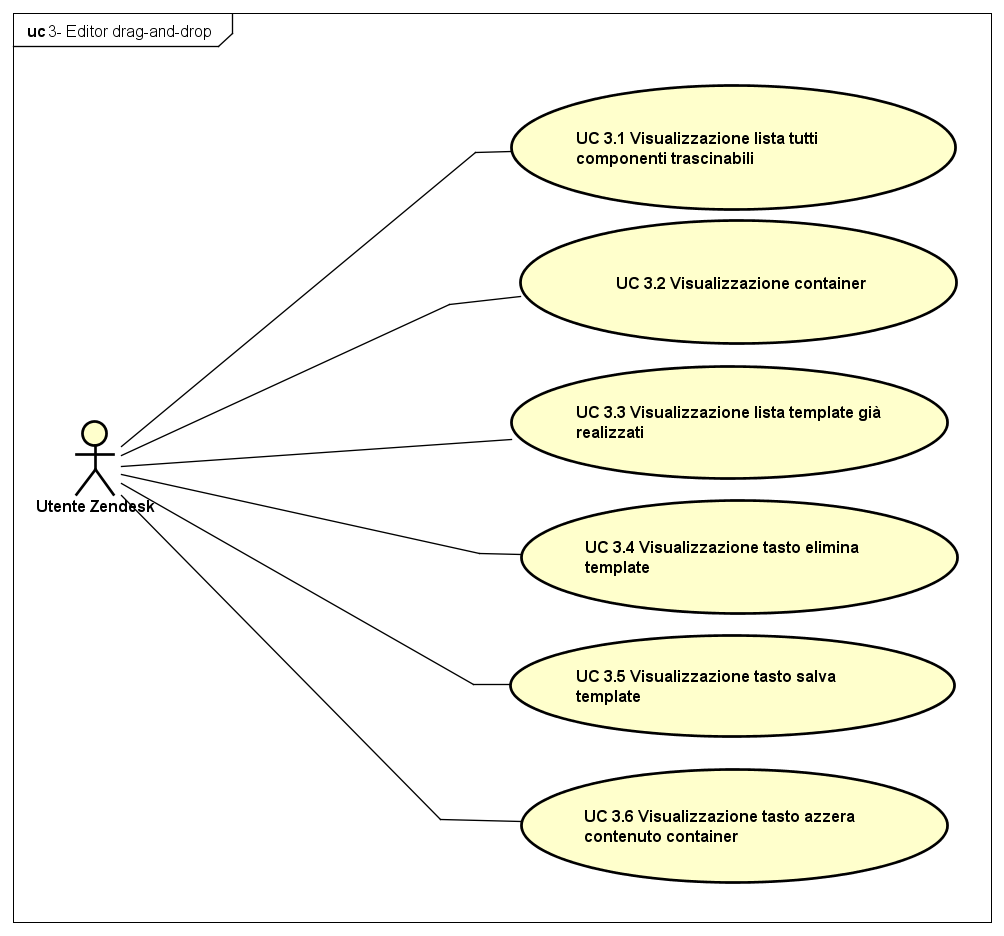
\includegraphics[width=1.2\columnwidth]{editor} 
	\caption{Editor realizzato }
\end{figure}
\begin{itemize}
	\item L'utente può trascinare qualsiasi elemento presente nei "componenti" nel container centrale;
	\item Il container visualizza a schermo il contenuto  HTML e CSS di ogni elemento trascinato in esso;
	\item Facendo doppio click su qualsiasi elemento presente nel container centrale è possibile modificare il suo contenuto oppure eliminarlo dal container;
	\item Gli elementi nel container possono essere ordinati in qualsiasi modo semplicemente facendo drag-and-drop;
	\item E' possibile azzerare il contenuto del container semplicemente cliccando il pulsante "Azzera";
	\item Una volta realizzato il template desiderato l'utente può salvarlo cliccando il pulsante "Aggiungi". Verrà chiesto all'utente di inserire il nome del template, inserendo il nome valido il template verrà automaticamente salvato sul database nosql di Amazon;
	\item A destra nell' "Elimina template" è possibile visualizzare tutti template realizzati e se necessario eliminarli semplicemente cliccano sull'icona "X".  
\end{itemize}
\section{Widget} 
Il widget permette all'agente di Zendesk di utilizzare i template realizzati nelle risposte verso clienti. 
  \begin{figure}[!h] 
  	\centering 
  	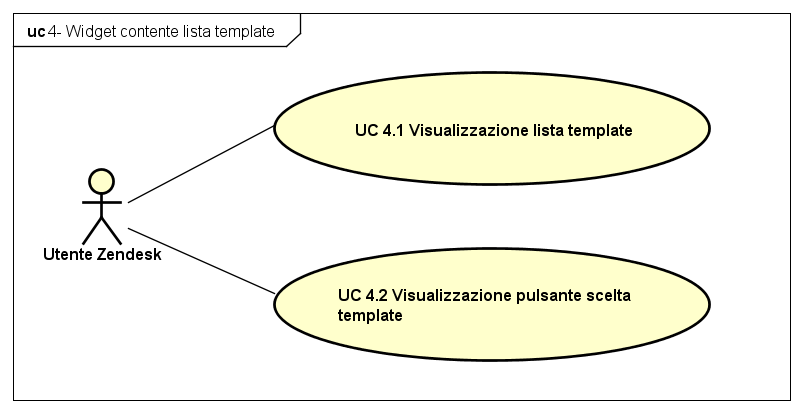
\includegraphics[width=1.2\columnwidth]{widget} 
  	\caption{Editor realizzato }
  \end{figure}
  \begin{itemize}
  	\item L'utente visualizza nel widget tutti i template realizzati;
  	\item L'utente può selezionare il template da utilizzare nella risposta;
  	\item Il template viene automaticamente aggiunto alla risposta. 
  \end{itemize}
\newpage
\section{Pagina di login}
Nella immagine di seguito viene visualizzata il form di login contenuto nella pagina di login. Una volta inseriti i dati corretti, viene automaticamente caricata la pagina degli amministratori. Se i dati inseriti non sono corretti, viene mostrato a schermo un messaggio di errore.
\begin{figure}[!h] 
	\centering 
	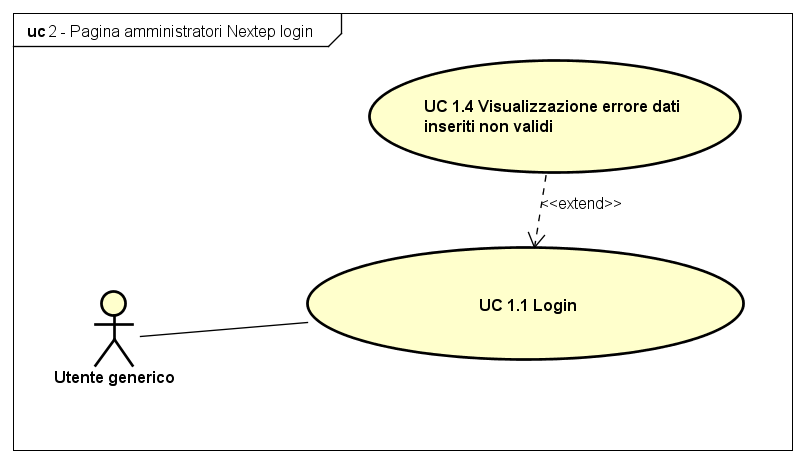
\includegraphics[width=0.8\columnwidth]{login} 
	\caption{Editor realizzato }
\end{figure}
\section{Pagina degli amministratori}
Nella immagine di seguito viene visualizzata la pagina degli amministratori. In questa pagina è possibile aggiungere e rimuovere un cliente di Nextep che utilizza oppure andrà ad utilizzare l'applicazione CS-Template.
\begin{figure}[!h] 
	\centering 
	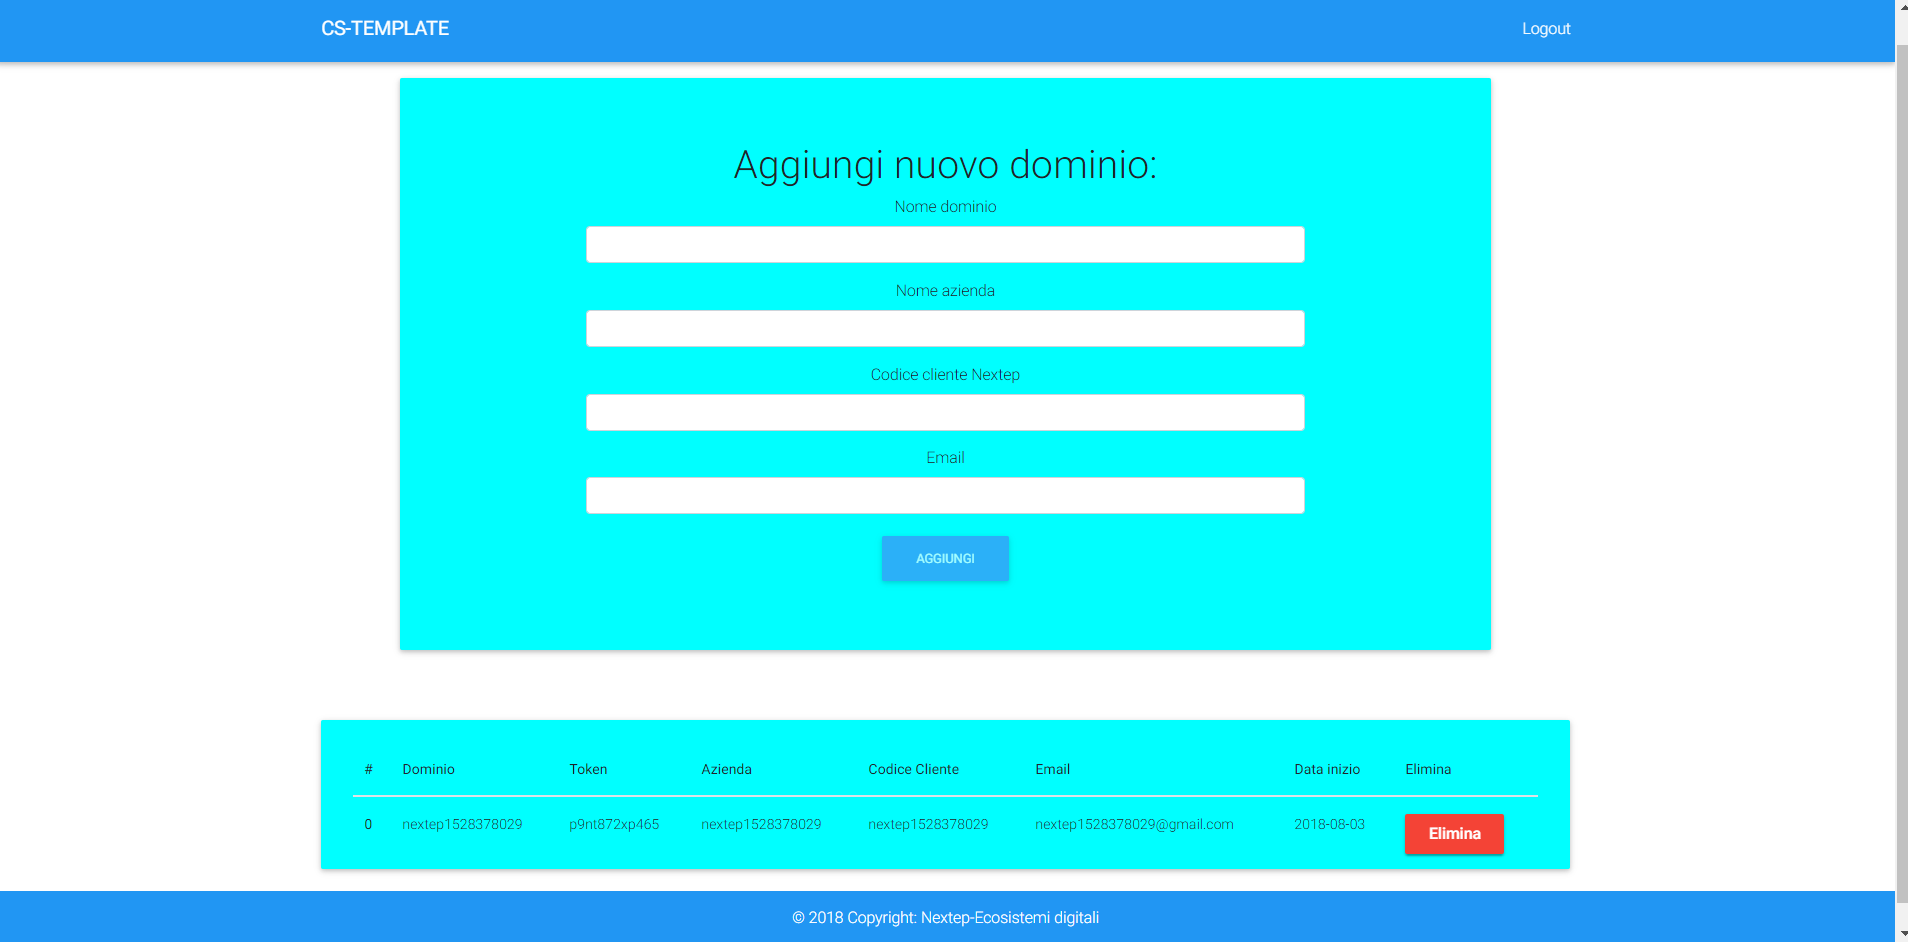
\includegraphics[width=1.2\columnwidth]{admin} 
	\caption{Editor realizzato }
\end{figure}

